\documentclass[a4paper,11pt]{article}
\usepackage[utf8]{inputenc}
\usepackage[T1]{fontenc}
\usepackage[norsk]{babel}
\usepackage{amsmath, amssymb, amsfonts}
\usepackage{graphicx}
\usepackage{booktabs}
\usepackage{siunitx}
\usepackage[hidelinks]{hyperref}
\usepackage{geometry}
\geometry{margin=2.5cm}

\title{Prosjekt 2 -- SIRS og Gruntvannsligninger}
\author{Kevin Dalland \\ Bachelor i Matematisk Modellering og Datavitenskap, OsloMet}
\date{\today}

\begin{document}
\maketitle
\tableofcontents
\newpage

\section{Innledning}
Dette prosjektet er todelt. I første del modelleres spredningen av en smittsom sykdom ved hjelp av en SIRS-modell (Susceptible–Infected–Recovered–Susceptible).  
Systemet løses både deterministisk ved ordinære differensialligninger og stokastisk ved Monte Carlo-simulering.  
I andre del brukes de numeriske metodene fra kurset til å løse gruntvannsligningene i to dimensjoner med et eksplisitt Lax–Friedrichs-skjema.

Målet er å sammenligne metodene, studere stabilitet og observere hvordan valg av parametere påvirker dynamikken i systemene.

\section{Del 1: SIRS-modell}
\subsection{Teori og ligninger}
SIRS-modellen beskrives av
\[
\begin{aligned}
S' &= cR - \frac{aSI}{N},\\
I' &= \frac{aSI}{N} - bI,\\
R' &= bI - cR,
\end{aligned}
\]
der $a$ er smittetakten, $b$ friskhetsraten, $c$ tap av immunitet, og $N=S+I+R$ er total populasjon.  
Ved å sette $S' = I' = R' = 0$ fås likevektene
\[
S^*=\frac{b}{a}, \qquad
I^*=\frac{c(a-b)}{a(b+c)}, \qquad
R^*=\frac{b(a-b)}{a(b+c)}.
\]
Endemisk likevekt eksisterer når $a>b$, dvs.\ når grunnreproduksjonstallet $\mathcal R_0 = a/b > 1$.

\subsection{Løsning med Runge--Kutta 4 (Del 1b)}
Differensialligningene løses numerisk med fjerdeordens Runge--Kutta-metode:
\[
y_{n+1}=y_n+\frac{h}{6}(k_1+2k_2+2k_3+k_4),
\]
der $k_1=f(t_n,y_n)$ osv.  
Parametrene er $a=1.0$, $c=0.1$ og $b\in\{\tfrac14,\tfrac12,\tfrac34,1\}$ med startverdier $S_0=300$, $I_0=100$, $R_0=0$ og $N=400$.

\begin{figure}[h!]
\centering
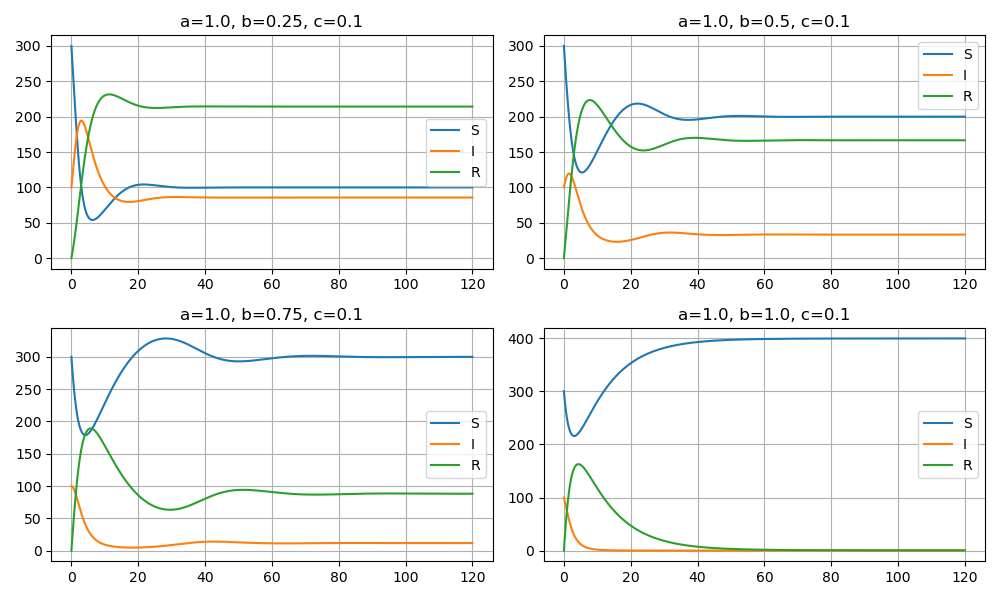
\includegraphics[width=0.8\textwidth]{figs/sirs_ode.png}
\caption{Utviklingen av $S$, $I$ og $R$ fra ODE-modellen for ulike verdier av $b$.}
\end{figure}

\subsection{Monte Carlo-simulering (Del 1c)}
For å inkludere stokastiske effekter simuleres overganger i hvert lite tidssteg $\Delta t$ med sannsynligheter
\[
P(S\to I)=\frac{aSI}{N}\Delta t, \qquad
P(I\to R)=bI\Delta t, \qquad
P(R\to S)=cR\Delta t,
\]
der $\Delta t = \min(4/(aN),\,1/(bN),\,1/(cN))$.  
Simuleringen repeteres $M$ ganger, og middel- og standardavvik beregnes.

\begin{figure}[h!]
\centering
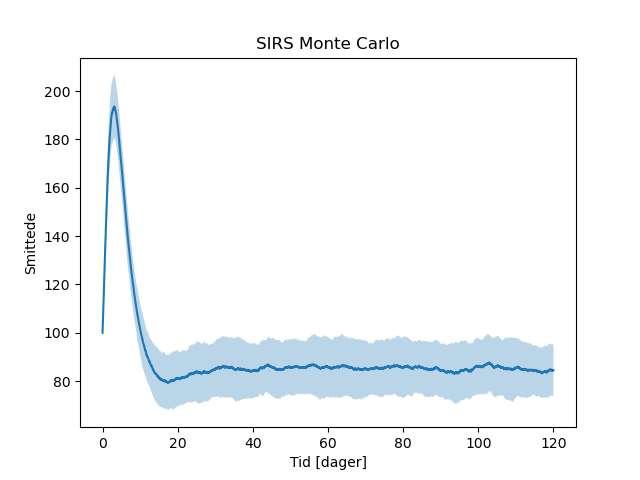
\includegraphics[width=0.8\textwidth]{figs/sirs_mc.png}
\caption{Gjennomsnittlig antall smittede (MC-simulering) med $\pm1$ standardavvik.}
\end{figure}

Resultatet viser at MC-gjennomsnittet følger den deterministiske løsningen tett når $N$ er stort, men med tydelige svingninger for små populasjoner.

\subsection{Vitaldynamikk (Del 1d)}
Modellen utvides med fødselsrate $e$, dødsrate $d$ og ekstra dødelighet $d_I$ for smittede:
\[
\begin{aligned}
S' &= cR - \frac{aSI}{N} - dS + eN,\\
I' &= \frac{aSI}{N} - bI - dI - d_I I,\\
R' &= bI - cR - dR.
\end{aligned}
\]
Dette gjør at totalbefolkningen $N(t)$ ikke er konstant.  
Systemet løses med samme RK4-metode, men med adaptivt tidssteg.

\begin{figure}[h!]
\centering
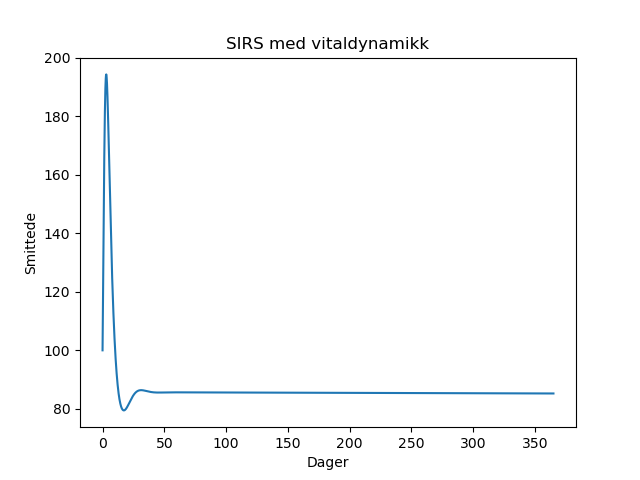
\includegraphics[width=0.8\textwidth]{figs/sirs_vital.png}
\caption{Utviklingen av $I(t)$ med vitaldynamikk. Fødsler og dødsfall stabiliserer systemet.}
\end{figure}

\subsection{Diskusjon}
For små $b$ (langsomme tilfriskninger) vokser smitten og når en endemisk likevekt.  
Når $b\ge a$ blir $I^*=0$, og sykdommen dør ut.  
Monte Carlo-modellen viser stokastiske svingninger rundt ODE-likevekten, mens vitaldynamikken innfører langsiktig stabilitet mot en bærekraftig befolkningsstørrelse.

\section{Del 2: Gruntvannsligninger}
\subsection{Modell og numerisk metode}
Gruntvannsligningene i 2D kan skrives som
\[
\partial_t Q + \partial_x F(Q) + \partial_y G(Q)=0,
\]
med
\[
Q=\begin{bmatrix} h\\hu\\hv \end{bmatrix},\quad
F(Q)=\begin{bmatrix} hu\\hu^2+\tfrac12 gh^2\\huv \end{bmatrix},\quad
G(Q)=\begin{bmatrix} hv\\huv\\hv^2+\tfrac12 gh^2 \end{bmatrix},
\]
hvor $h$ er vannhøyde og $(u,v)$ hastighetskomponenter.

Diskretisering (Lax--Friedrichs-aktig FTCS):
\[
Q^{n+1}_{i,j}
=\tfrac14(Q^n_{i+1,j}+Q^n_{i-1,j}+Q^n_{i,j+1}+Q^n_{i,j-1})
-\frac{\Delta t}{2\Delta x}\big(F^n_{i+1,j}-F^n_{i-1,j}\big)
-\frac{\Delta t}{2\Delta y}\big(G^n_{i,j+1}-G^n_{i,j-1}\big).
\]
Tidssteget tilfredsstiller CFL-betingelsen
\[
\Delta t \le \min\!\left(\frac{\Delta x}{\max(|u|+\sqrt{gh})},\,\frac{\Delta y}{\max(|v|+\sqrt{gh})}\right).
\]

\subsection{Dam-brudd (Del 2a--c)}
Initialtilstanden består av et sirkulært område med høyere vannhøyde $h_D$ omgitt av lavere nivå $h_S$:
\[
h(x,y)=
\begin{cases}
h_D, & (x-L_x/2)^2+(y-L_y/2)^2 < R^2,\\
h_S, & \text{ellers.}
\end{cases}
\]
Periodiske, Neumann- og Dirichlet-randbetingelser testes.

\begin{figure}[h!]
\centering
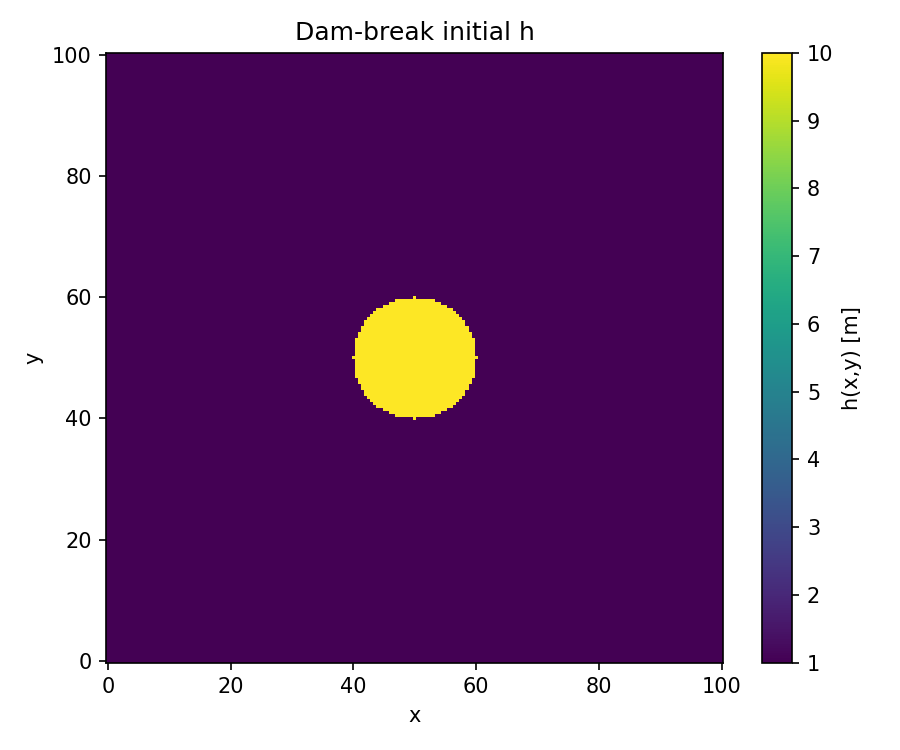
\includegraphics[width=0.8\textwidth]{figs/shallow_init.png}
\caption{Initial vannhøyde for dam-brudd-testen.}
\end{figure}

\begin{figure}[h!]
\centering
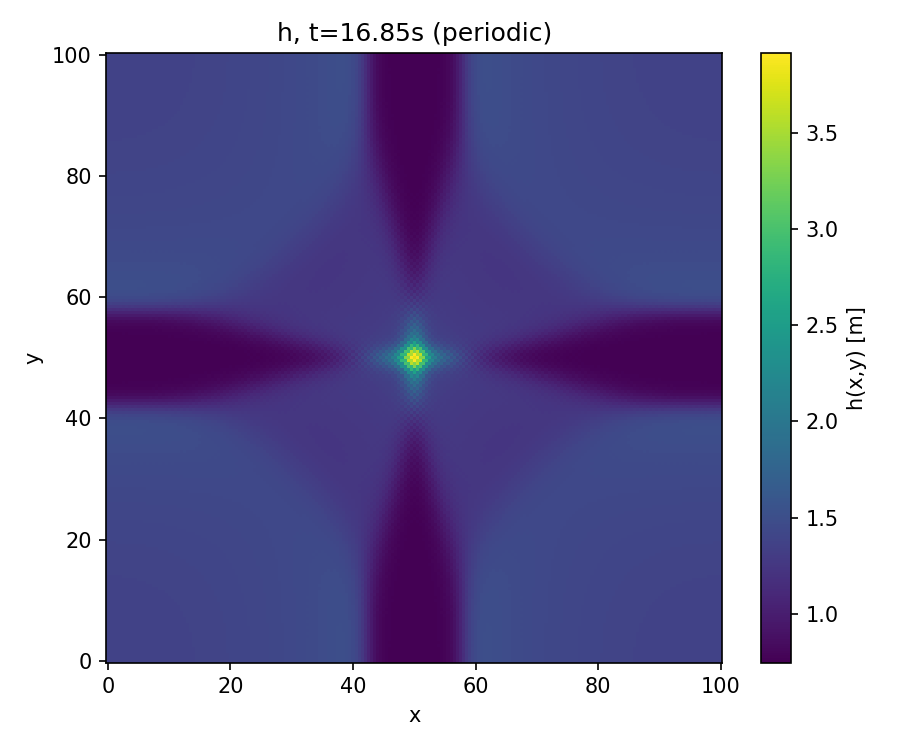
\includegraphics[width=0.8\textwidth]{figs/shallow_periodic_tend.png}
\caption{Sluttstadiet for periodiske randbetingelser.}
\end{figure}

\subsection{Stor skala (Del 2e)}
For en større modell med $(L_x,L_y)=(1000\,\mathrm{km},1000\,\mathrm{km})$ og bakgrunnshøyde $H=100\,\mathrm{m}$ brukes
\[
h_0(x,y)=H + \exp\!\Big[-\frac{(x-L_x/2)^2}{2(0.05L_x)^2}-\frac{(y-L_y/4)^2}{2(0.05L_y)^2}\Big]
          + \exp\!\Big[-\frac{(x-L_x/4)^2}{2(0.05L_x)^2}-\frac{(y-3L_y/4)^2}{2(0.05L_y)^2}\Big].
\]

\begin{figure}[h!]
\centering
\includegraphics[width=0.8\textwidth]{figs/shallow_neumann_tend.png}
\caption{Bølgespredning i stor skala med Neumann-randbetingelser.}
\end{figure}

\subsection{Diskusjon}
Skjemaet bevarer massen godt og er stabilt for CFL ≈ 0.45.  
Numerisk diffusjon demper høye frekvenser, men gir jevn bølgespredning.  
Ved Dirichlet-rand observeres refleksjon, mens Neumann tillater fri utstrømning.

\section{Konklusjon}
Prosjektet illustrerer forskjeller mellom deterministiske og stokastiske modeller, samt hvordan eksplisitte metoder kan brukes på PDE-systemer.  
SIRS-modellen viser hvordan smitteparametere styrer likevekten, mens gruntvannseksperimentet viser bølgedynamikk og numerisk stabilitet under ulike randbetingelser.

\section*{Reproduserbarhet}
Koden er skrevet i Python 3.12 med bibliotekene NumPy 1.26, Matplotlib 3.9, SciPy 1.13 og Numba 0.59.  
Kjør følgende kommandoer for å generere figurene:
\begin{verbatim}
python kode/sirs_model.py
python kode/sirs_mc.py
python kode/sirs_vital.py
python kode/shallow_water.py --bc periodic
\end{verbatim}

\bibliographystyle{plain}
\bibliography{refs}
\end{document}

